\section{Named Entity Extraction} 

Extracting named entities from texts and representing them as nodes in knowledge graphs generally, involves three main
tasks: Named Entity Recognition (NER), Named Entity Disambiguation (NED) and Named Entity Linking (NEL). 

\subsection{Named Entity Recognition (NER)} \label{named_ents}

\textbf{Named entity recognition (NER)} is a process which extracts and classifies named entities of a certain (sometimes pre-defined) types
from an unstructured text. \hyperlink{9}{[9]} 

First, it identifies the 'names' of the entities from the tokens (pre-processed) which is commonly done by BIO (beginning-inside-outside) tagging and POS tags. It then performs sequence labelling (assigning labels/tags to each element of an input sequence) and classify entities into the predefined types such person, location, organisation etc. as seen in Figure 2. \hyperlink{9}{[9]}

A popular sequence labelling model is \textbf{Conditional Random Fields }(CRF). These are "discriminative models" and generally outperform other Markov Models and such as Hidden Markov Models (HMM) as they are better able to cope with unseen tokens/words as well as Maximum Entropy Markov Models (MEMM) as they do not have labelling bias. \hyperlink{13}{[13]}

They work by maximising the log-likelihood of the posterior distribution P(S|O) where S is  the output label sequence and O is the observed input sequence. Let S' denote the correct label sequence: 

$ S' = \argmax_{S} P (S|O) $

Therefore, it is fairly simple to determine output label sequence as it will be the one with the highest posterior probability. E.g. P([Per, Org, Org] | [Obama, UN, Congress]) will have a much higher probability than  P([Loc, Loc, Loc] | [Obama, UN, Congress]). \hyperlink{13}{[13]} 

The NER models are usually trained on specific domains and thereby only extract certain types of entities (pre-defined types such as PER, LOC, ORG), thereby making them domain-dependent.



% \subsection{NER Approaches}

% \begin{enumerate}
%     \item \textbf{Rule $/$ knowledge-based approaches:} These methods depend on pre-defined (hand-crafted rules). The primary advantage is the lack of need for annotated training data as they focus on lexical representation and resources. These can be useful for domain-specific uses as they are rules are exhaustive and can help extract model-specific knowledge, resulting in high precision model. A drawback, however, is they will perform poorly when extended to other domains, and poor generalisability means constructing and maintaining lexicon resources for many domains is costly.

%     \item \textbf{Learning-based approaches:} These methods replace the human-curated rules. These methods can be further classed
% into three types: supervised, semi-supervised, and unsupervised. Supervised and semi-supervised methods,
% require the ML model to be trained on the input input given the corresponding output data to learn the features mapping the inputs to the outputs. Common examples to model the classifiers include  Hidden Markov Models (HMM), Support Vector Machines (SVM), and
% Conditional Random Fields (CRF). The type of classifier can have an effect on the accuracy of the NER task. For instance, SVM and HMM do not consider the dependencies among words. The unsupervised,
% bootstrapped methods are generally more automated in that they do not require an expansive training set (seeds) and but are less common. 
% (seeds). \hyperlink{9}{[9]}

% \item \textbf{Feature-inferring neural-network approaches:} Like learning-based approaches they incorporate machine learning techniques, however, they automatically infer the features by using deep neural networks (DNNs) such as LSTM. Reportedly, \hyperlink{9}{[9]}, they generally outperform the other approaches. They are able to perform feature extraction in the lower layers of the network and use these to train the classifier. The advantage is that they do not require seeds, ontologies or any domain-specific lexicons and are therefore domain-independent making them more robust. However, they do require huge datasets to build a decent model.  \hyperlink{9}{[9]}
% \end{enumerate}


\subsection{Named Entity Disambiguation (NED)}

\textbf{Named Entity Disambiguation (NED)}: As seen in \textbf{Figure 2}, NER might not always be able to classify a named identity due to it having a different meaning in different contexts. This is why named entity disambiguation is crucial to determine which
named entity a mention refers to; For instance, ‘Trump’ can refer to either a person, a corporation or a building. \hyperlink{9}{[9]}

This is where context representation comes into play which uses the knowledge base to learn about the entities. In order to disambiguate words, models use as textual and structural representations. Examples of textual representations are bag-of-words (BoW) approach where for each ambiguous entity, it keeps track of all concatenated paragraphs the entity was mentioned in and compares them with a target article, selecting the best matching. Vector space model and cosine similarity can be used for text comparison and TF-ICF (term frequency-inverse corpus frequency, more efficient version of TF-IDF  \hyperlink{12}{[12]}) for weighting individual terms.  \hyperlink{11}{[11]} 

In structural representation methods, the context can be represented as the entirely of the text.
An example in \hyperlink{11}{[11] (p.7)} shows that for the sentence: "Michael Bloomberg is the mayor of New York", their algorithm correctly identifies New York in USA instead of London as Michael Bloomberg co‐occurs in the same paragraph New York city in the USA in the KB significantly more "(88 times) than with the New York in England (0 times)". Quantifying  the impact of co‐occurrences, can be done by using incidence matrix represents a weighted graph where weights are the co‐occurrence $|$P(e$_{i}$,s,e$_{j}$,t)$|$ i.e. count of paragraphs, where two different entities e$_{i}$ and e$_{j}$ were mentioned together in two different sentence forms (s $\neq$ t). \hyperlink{11}{[11]}

% \subsection{NED Approaches}

% NED approaches can be divided into two types: 
% \begin{enumerate}
%     \item \textbf{Traditional approaches:} which use hand-crafted pre-defined features to compute the measure of similarity between the candidate entities and mentions (from the text). These are generally of two types:
%     \begin{enumerate}
%     % https://aclanthology.org/K16-1026.pdf
%         \item Independent/local approaches rank the candidate entries based on lexical similarity and empirical co-occurrence with their corresponding mentions using techniques such BOW (bag of words) based on cosine similarity. Here, Entity disambiguation is modelled as a ranking problem, where each entity is disambiguated independently and the one with the highest probability/score calculated by hand-designed features from the mention's context. These methods can perform poorly as they fail to consider the interactions between the entity mentions within the same document. \hyperlink{9}{[9]}\hyperlink{15}{[15]}
        

%     \item Collective approaches exploit the idea that entities mentioned in the same area of a text (say a document) is likely about the same topic and therefore, establish a semantic relationship between any co-occurring entities. Commonly a probabilistic graph-based approach is adopted to build entity-mention pairs to establish a relationship between candidate entries. Random walk-through and page-rank algorithms can be applied to establish a well-matched entity group. \hyperlink{9}{[9]}

%     \end{enumerate}
    

% \item NN approaches: These have become increasingly popular and use neural networks to disambiguate entities based on their context. They can use models that use continuous vector spaces and generally use Embedding-based features (which can extract syntactic and
% semantic relations between words). Embedding-based
% features learn continuous vector representation for words (from unlabelled text) based on context or predict context based on surrounding words. (Refer to Section 2.6.1) They have much better performance than BoW-based features. \hyperlink{15}{[15]}. Deep neural networks (DNNs) can automatically infer any latent semantic features (feature engineering). This approach, therefore, results in a more generalisable model and results in higher accuracy.
    
% \end{enumerate}

% \subsection{Named Entity Linking (NEL)}

% \textbf{Named Entity Linking (NEL)} aims to provide a standard IRI for each disambiguated entity as described in a Knowledge Base (e.g. Linked Open Data (LOD) Cloud). Entity mentions are annotated by some NER algorithms, but they are restricted to the pre-defined types (such as persons, locations, organizations). \hyperlink{9}{[9]} Knowledge base hosts millions of entities and therefore NEL can be used to ground mentions of entities in some text to a central KB. An example mentioned in this \hyperlink{14}{paper [14]}  highlights this: 'David Murray recruited from Positive Black Soul' grounds Wikipedia articles for David Murray (saxophonist) but not the David Murray (musician) (disambiguation based on context) and Positive Black Soul. 

% NEL has three main sub-tasks:

% \begin{enumerate}
%     \item Candidate-entity generation: tries to extract all possible entities in the knowledge base (KB) that could potentially refer to an entity mention in the text. This can be done by dictionary-based approaches, supervised learning of surface (sentence) form expansion from documents or probability-based approaches. 
    
%     \item Candidate-entity ranking: this step resembles disambiguation as seen in NED. This involves ranking candidate entries and retrieving the one with the highest probability for a target mention. The ranking can be established  via supervised methods (which include graph-based, model ensemble and probabilistic approaches) as well as unsupervised methods (which include Vector-Spaced Model and Information Retrieval based approaches.) \hyperlink{9}{[9]}
    
%     \item NIL clustering: handles those mentions in the text that have no matches with any entities in the knowledge base (KB). Of the three steps, this one is often not developed extensively. This can be implemented using string matching (grouping entities based on the string),  graph-based approaches (use a semantic entity graph) and hierarchical agglomerative clustering (based on minimising a distance metric). \hyperlink{9}{[9]}

% \end{enumerate}

% \subsection{NEL Approaches}

% NEL approaches can be classified into two groups: 

% \begin{enumerate}
%     \item Disambiguation-only approach: This mainly focuses on the second NEL step. These work under the assumption that all the mentions and candidates have been identified/ generated and focus on disambiguation the mentions from the entities and establishing a relationship between them by linking them. \hyperlink{9}{[9]}
    
%     \item End-to-end approach: These approaches directly get text as input and perform NER, Candidate entity extraction and ranking from the input text and finally linking them with their respective entities in the knowledge graph (KG). These often use Deep NN and primary components can include entity embeddings, context-dependent embeddings of mentions (e.g. ELMo discussed in Section 2.6.2),  and a probabilistic map linking entities and mentions. An example of the end-to-end NEL approach is the Neural Collective Entity Linking (NCEL) model which uses Graph Convolutional Networks on entity-subgraphs. \hyperlink{9}{[9]}

%     \end{enumerate}
    
    
% \begin{figure}[H]
% \centering
% 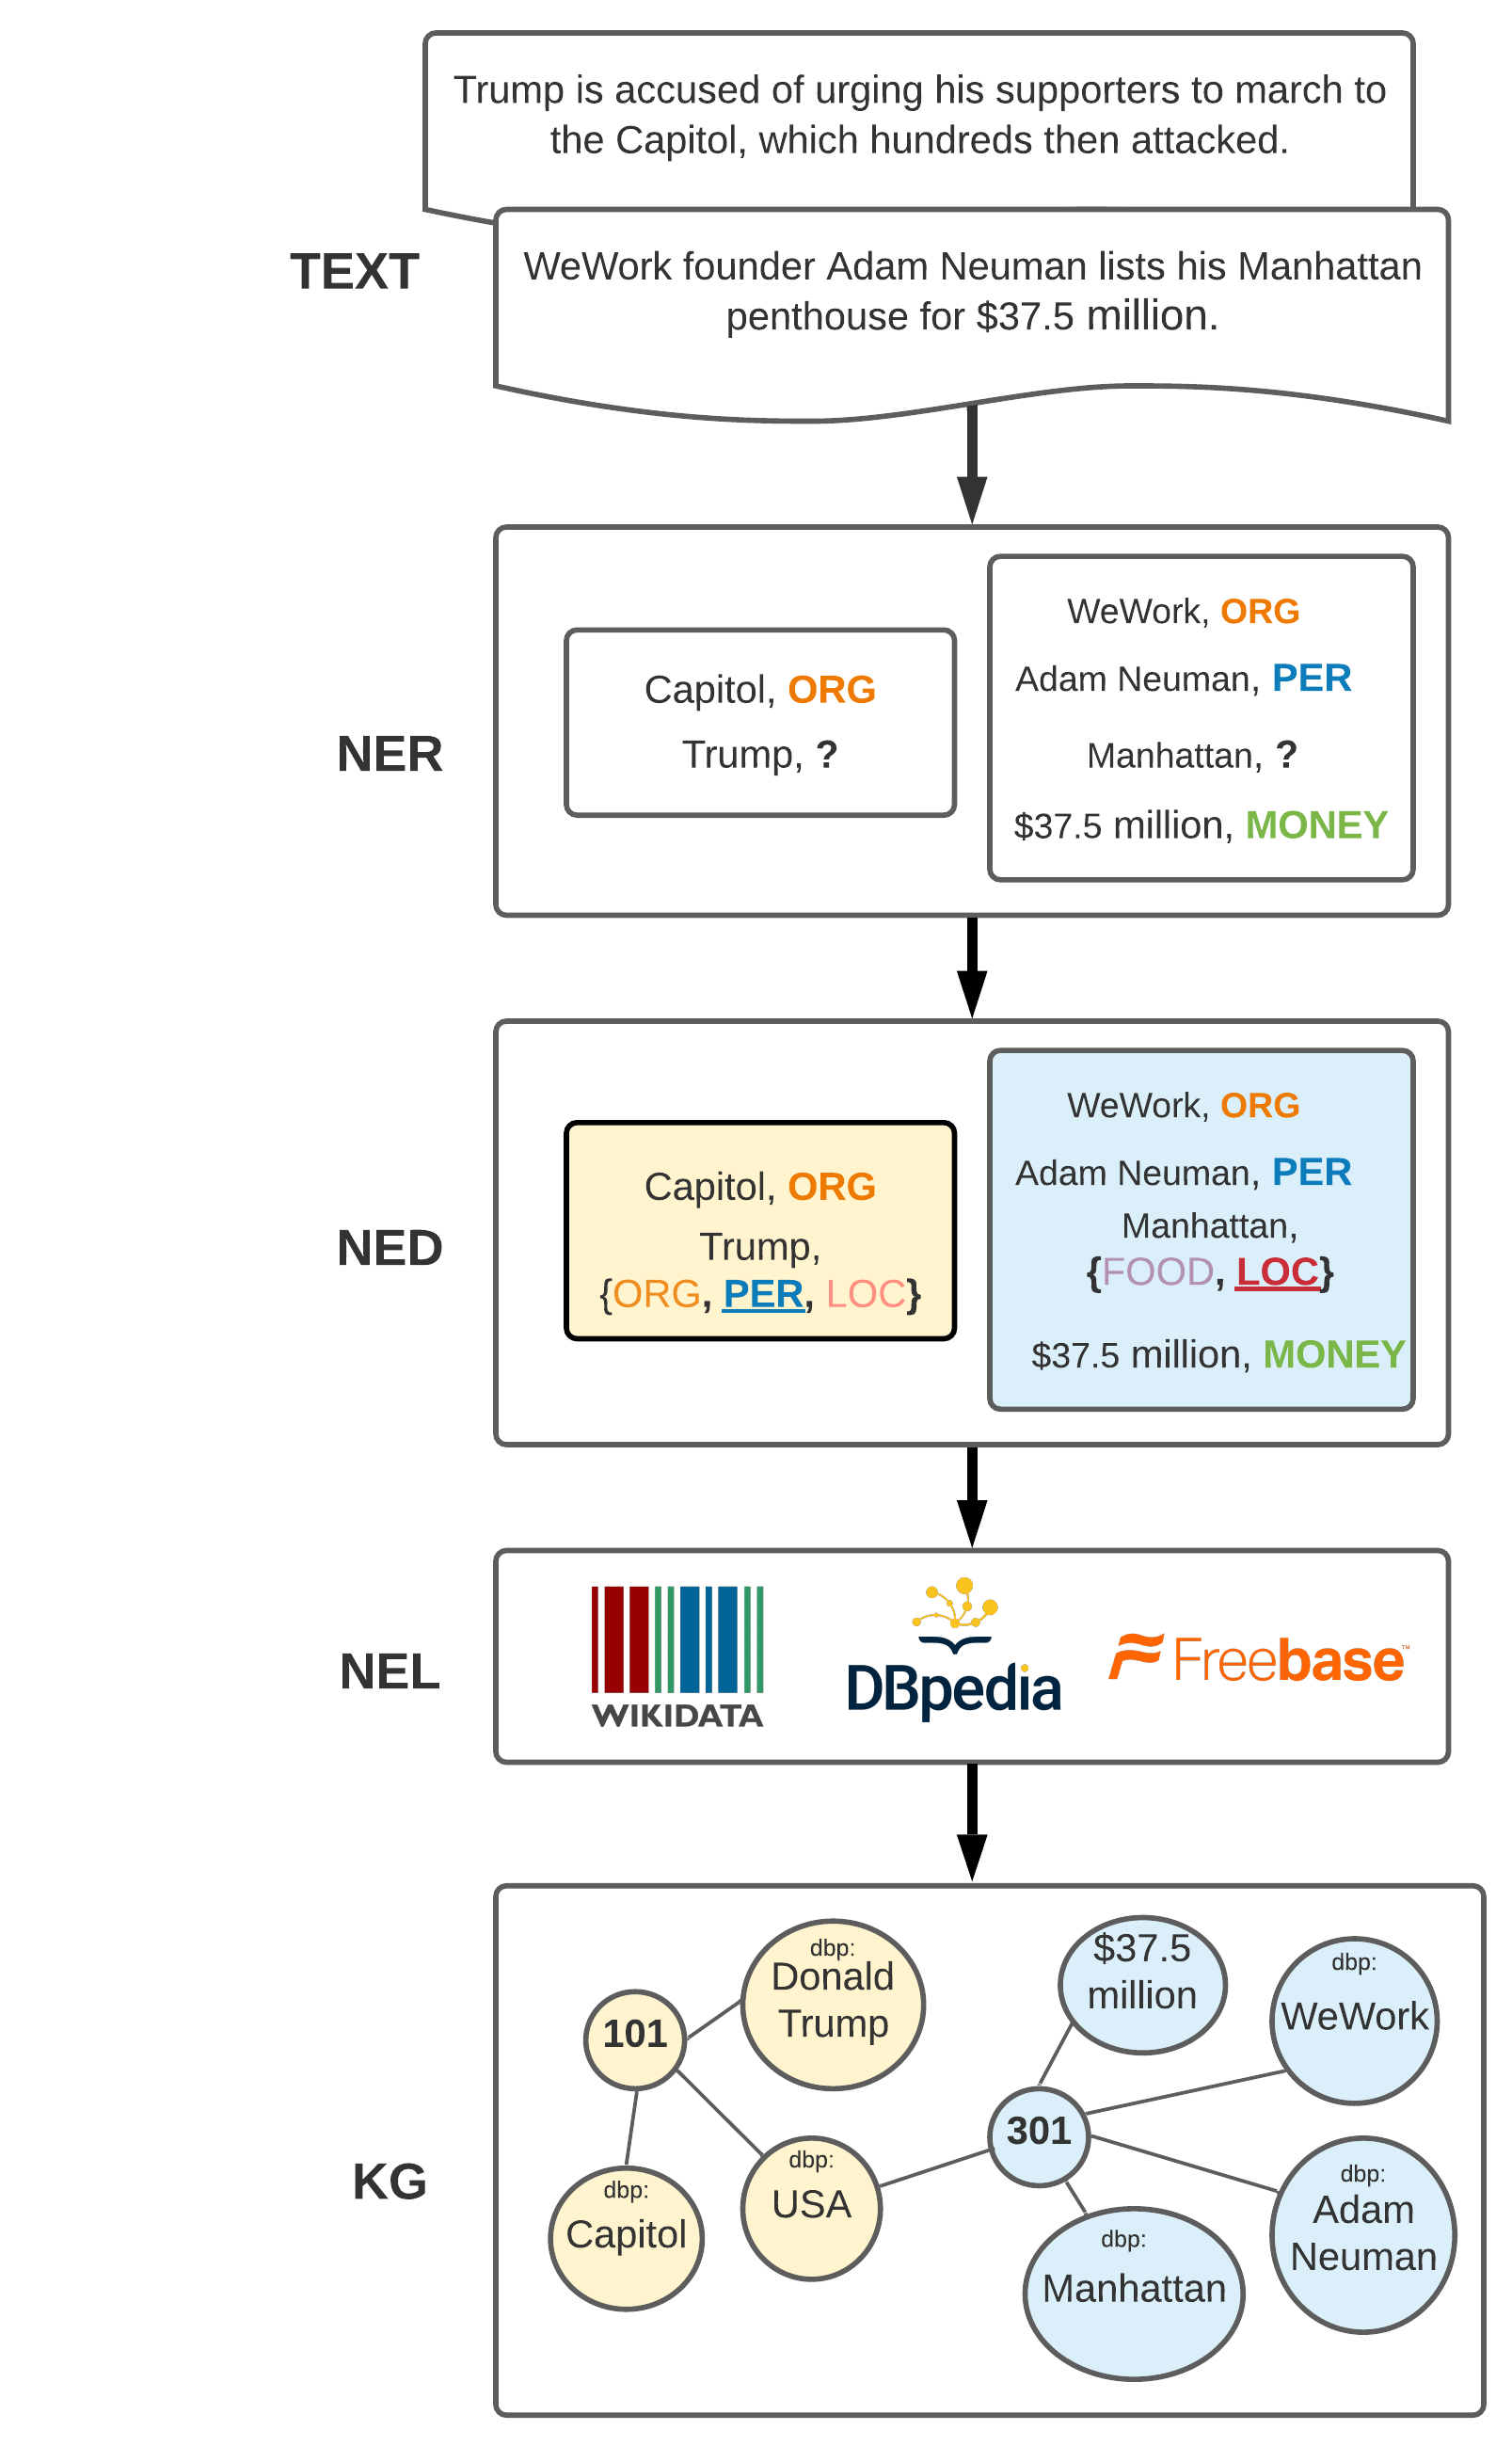
\includegraphics[scale = 0.2]{images/pipeline.png}
% \caption{Named Entity Extraction}
% \end{figure}

% % ----------------------------------------------- SENTIMENT ANALYSIS -------------------------------------------------------

